%\VignetteIndexEntry{Analysis of alternative splicing using ASpli}
%\VignetteKeywords{Alternative splicing analysis}
%\VignettePackage{ASpli}
\documentclass{article}
<<style, echo=FALSE, results=tex>>=
BiocStyle::latex()
options(continue=" ")
@

\usepackage{verbatim} 
\usepackage{caption} 
\usepackage{cite}
\usepackage{subcaption}

\title{\texttt{ASpli}: An integrative R package for analysing alternative 
  splicing using RNAseq}

\author{Estefania Mancini, Javier Iserte, Marcelo Yanovsky, Ariel Chernomoretz}

\begin{document}

\SweaveOpts{concordance=TRUE}

\maketitle

\tableofcontents

\section{Introduction}

Alternative splicing (AS) is a common mechanism of post-transcriptional gene 
regulation in eukaryotic organisms that expands the functional and regulatory 
diversity of a single gene by generating multiple mRNA isoforms that encode 
structurally and functionally distinct proteins. The development of novel 
high-throughput sequencing methods for RNA (RNA-Seq) has provided a powerful 
means of studying AS under multiple conditions and in a genome-wide manner 
\cite{pmid24549677}. However, using RNA-seq to study changes in AS under 
different experimental conditions is not trivial. 
In this vignette, we describe how to use ASpli, an integrative and user-friendly
R package that facilitates the analysis of changes in both annotated and novel 
AS events. This package combines statistical information from exon, intron, and 
splice junction differential usage (p-value, FDR), with information from splice 
junction reads to calculate differences in the percentage of exon inclusion 
($\Delta$PSI) and intron retention ($\Delta$PIR). The proposed methodology 
reliably reflect the magnitude of changes in the relative abundance of different 
annotated and novel AS events. This method can be used to analyze both simple 
and complex experimental designs involving multiple experimental conditions.

\section{Getting started}

BAM files of each sample and gene annotation are mandatory. Make sure all files 
use the same coordinate system. It is a good practice to organize all required 
files (or symbolic links of them) together into the  working directory.

\subsection{Installation}
ASpli is available at Bioconductor site and can be downloaded using
\texttt{biocLite()}:
<<installation, echo=TRUE, eval=FALSE>>=
source("https://www.bioconductor.org/biocLite.R")
biocLite("ASpli")
@
<<loadASpli, echo=TRUE, eval=TRUE>>=
library(ASpli)
@
 
\texttt{biocLite()} will take care of installing all the packages that ASpli 
depends on e.g. edgeR, GenomicFeatures, GenomicRanges, GenomicAlignments, Gviz, 
and other R package required. Some package depends on operating system packages,
like \texttt{curl} that are not installed automatically, and should be installed
by the user.

\subsection{ Building a \texttt{TxDb} of your genome }
Gene annotation is handled using \texttt{TxDb} objects, which are provided by
\texttt{GenomicFeatures} package. The building of a \texttt{TxDb} object might 
be time consuming, depending on the size of your genome. If a \texttt{TxDb} has
been already created, we strongly recommend saving it as a \texttt{sqlite} file
and reloading it any time the analysis is run. The \texttt{GenomicFeatures} 
package provides functions to create TxDb objects based on data downloaded from
UCSC Genome Bioinformatics, BioMart or gff/gtf files. See "Creating New TxDb 
Objects or Packages" in the \texttt{GenomicFeatures} vignette for more details.
In this example, a TxDb is built from a gtf file:

<<makeTx, echo=TRUE, eval=FALSE>>=
library(GenomicFeatures)
TxDb <- makeTxDbFromGFF(
  file="genes.gtf",
  format="gtf")
@



\section{Running \texttt{ASpli}}

The workflow intended to be used with \texttt{ASpli} is divided in four
independent steps (Figure \ref{fig:ASpliStructure}). For each of these steps
ASpli provides a single or few functions to use:
\begin{enumerate}
  \item Feature extraction: \texttt{ binGenome() }
  \item Read counting: \texttt{ readCounts() }
  \item Alternative splicing discovery using junctions: \texttt{ AsDiscover() }
  \item DE and DU estimation \texttt{ DUreport(), junctionDUReport() and
  DUreportBinSplice() })
\end{enumerate}

At each step it is possible to export results in a friendly manner. 
See Section "3.5 Outputs and results" for more details.

\begin{figure}[ht!]
\centering
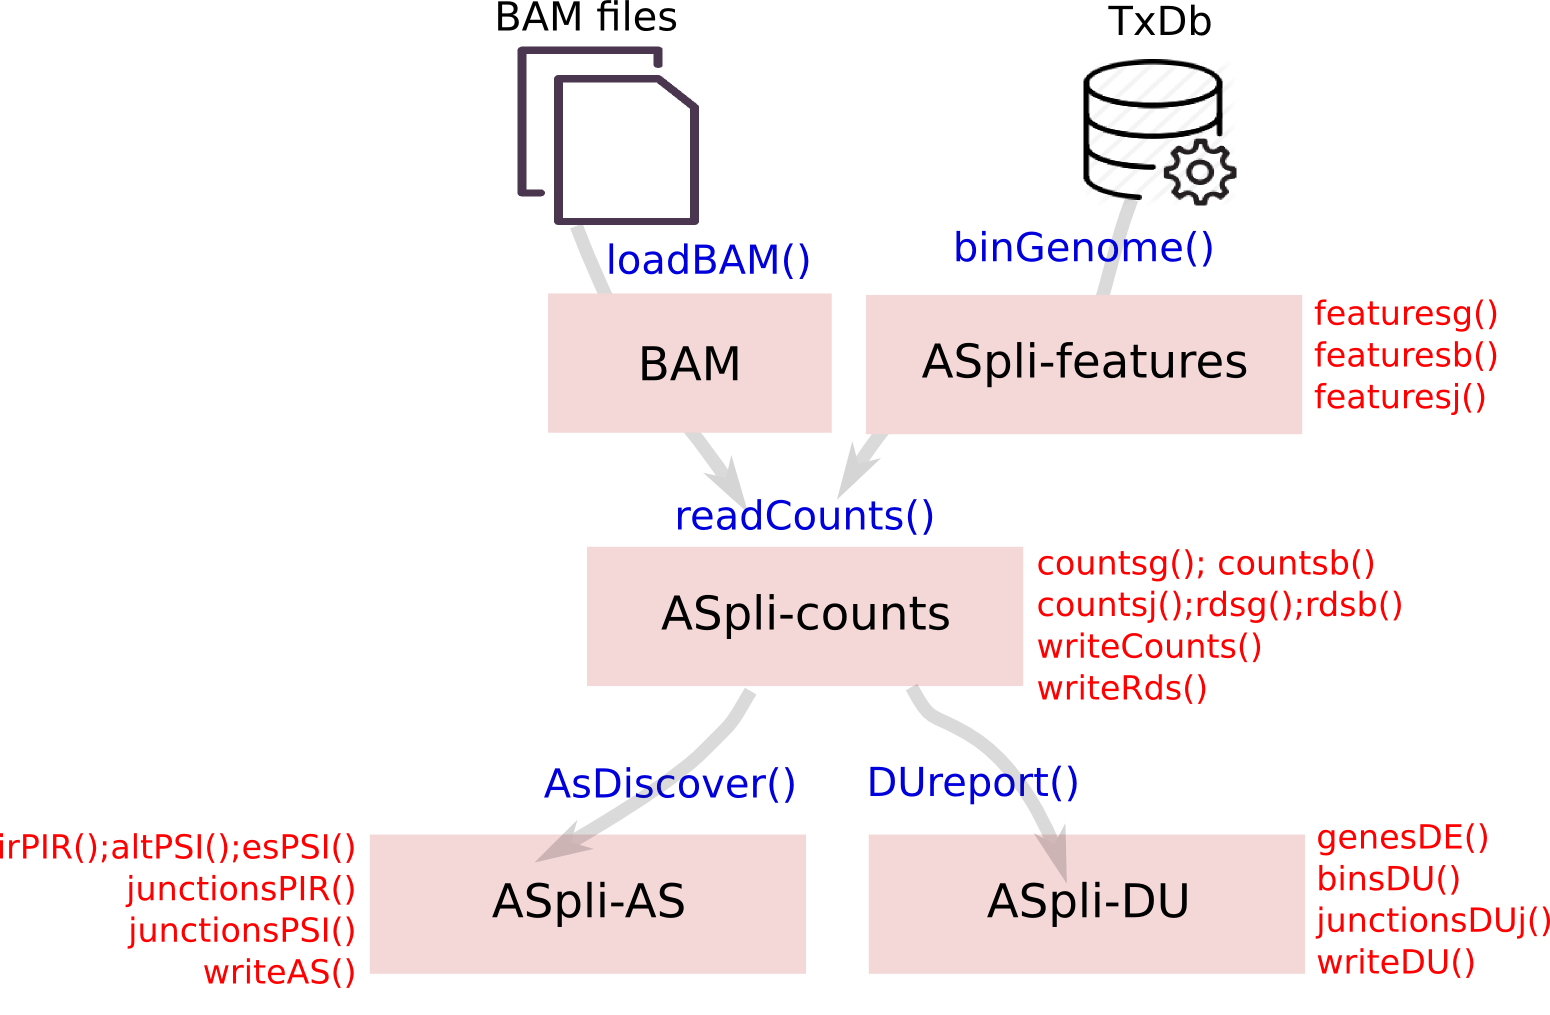
\includegraphics[width=0.5\textwidth]{wf.png}
\caption{Objects (squares) and methods (in blue) in ASpli package.  
  Accesors and write methods are in red. }
\label{fig:ASpliStructure}
\end{figure}

\subsection{ To BIN or not to BIN } %1
Sub-genic features such as exons and introns are analyzed using existing
annotations by splitting the genome into non-overlapping features called bins, 
as described previously for DEXSeq \cite{pmid22722343}. Exon and intron 
coordinates are then extracted from the annotation, but only those from 
multi-exonic genes are saved for further evaluation. When more than one isoform 
exists, some exons and introns will overlap. Exons and introns are then 
subdivided into new features called exon and intron bins, and are then 
classified into exclusively exonic bins, exclusively intronic bins, or 
alternative splicing (AS) bins (See Figure \ref{fig:binDefinition}). Each AS bin
is then assigned to a kind of splicing event. 

\begin{itemize}
\item \textbf {ES} (Exon skipping)
\item \textbf {IR} (Intron retention)
\item \textbf {ALt5'SS} Alternative five prime splicing site
\item \textbf {ALt3'SS} Alternative three prime splicing site
\item "*" (ES*, IR*, AltSS*) For bins involved in more than one AS event type
\item \textbf {external}: beginning or end of a transcript
\end{itemize}

Annotated junctions from all the transcripts are also reported. Junction 
coordinates are defined as the last position of the five prime exon (donor 
position) and first position of the three prime exon (acceptor).

Subgenic features are labeled as follow (hypothetical GeneAAA):
\begin{itemize}
\item \textbf{GeneAAA:E001}: defines first exonic bin
\item \textbf{GeneAAA:I001}: defines first intronic bin
\item \textbf{GeneAAA:Io001}: defines first original intron before being divided
\item \textbf{GeneAAA:J001}: defines first junction
\end{itemize}

Bins and junctions are labeled always in  5' to 3' sense of the plus strand of
the reference sequence. This implies that  bins and junctions with lower 
numbering are always closer to the 5' of that strand.
  
\begin{figure}[ht!]
\centering
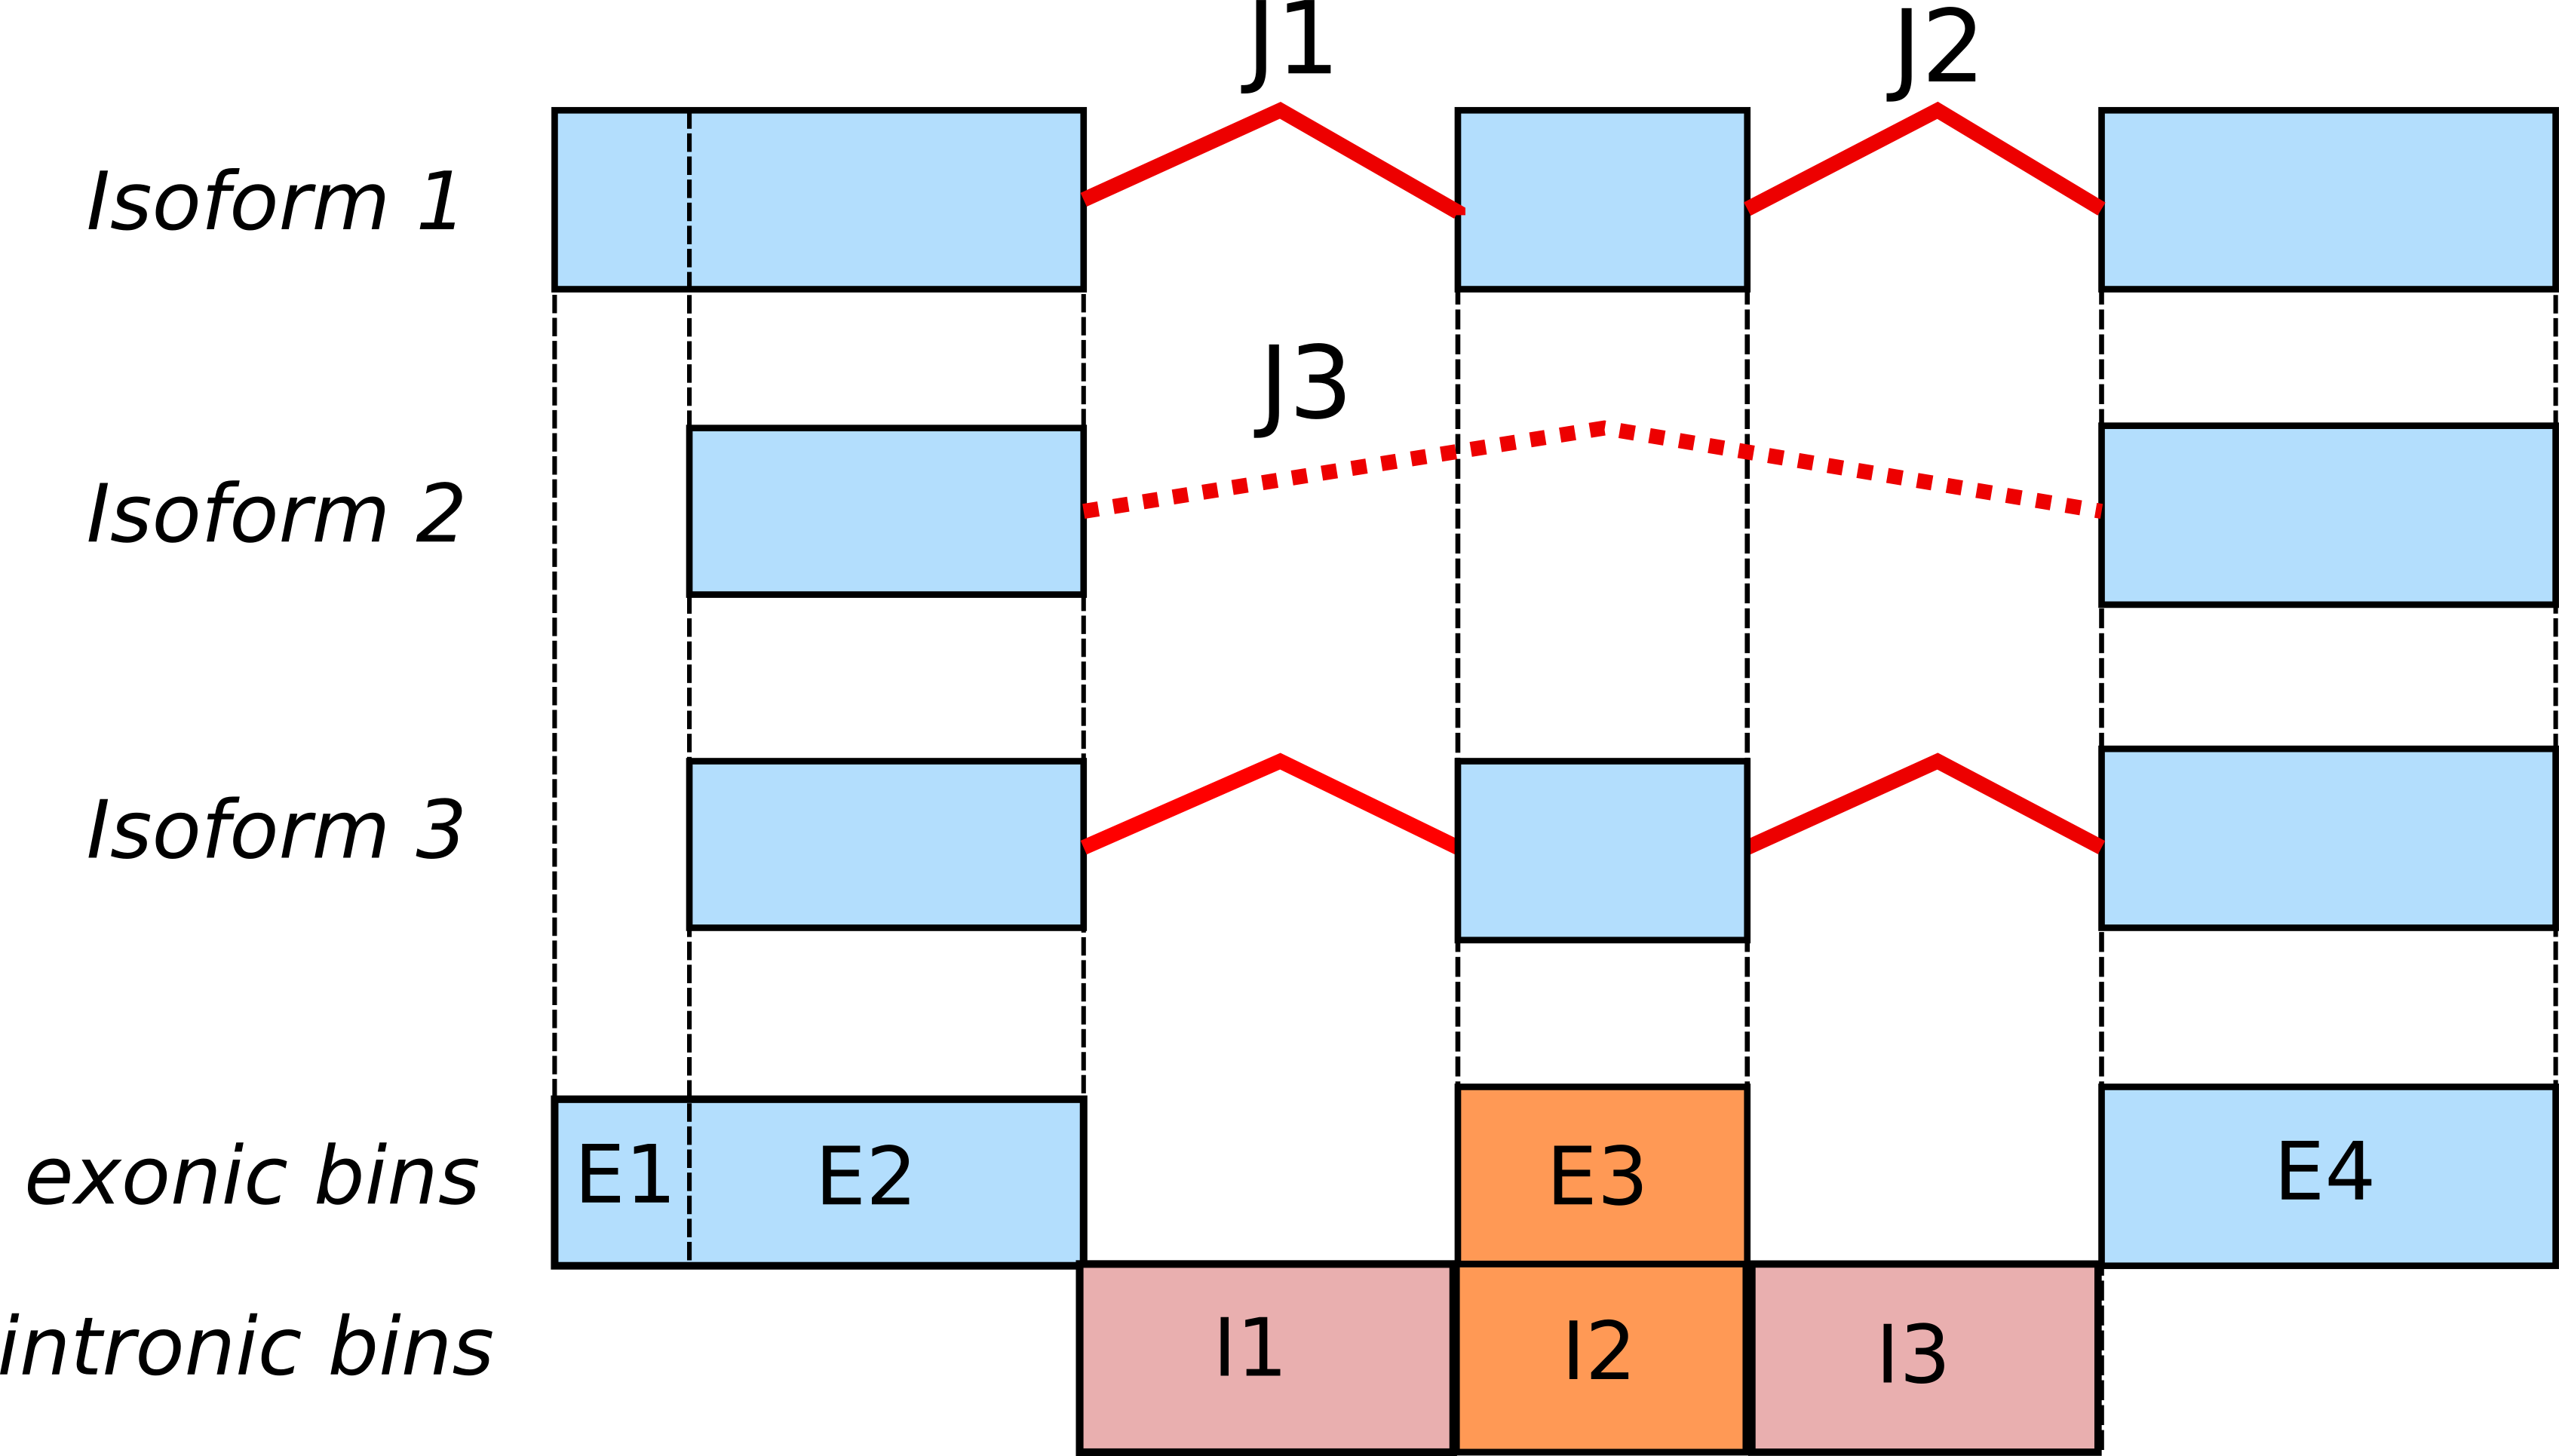
\includegraphics[width=0.3\textwidth]{binDefinition.png}
\caption{Scheme of resulting bins from a gene with two hypothetical transcripts. 
Those bins that are exonic or intronic at the same time are named \textit{AS
bins}. The junctions repertoire is also shown.
}
\label{fig:binDefinition}
\end{figure}

The \texttt{binGenome} method allows us to  extract genome coordinates at the 
gene, exon, intron and junction level and returns an object of class 
\texttt{ASpliFeatures}. Then, features cordinates could be extractd using their 
accesors:

<<binGenome, echo=TRUE, eval=FALSE>>=
features <- binGenome(TxDb) 
GenesCoord <- featuresg(features)
BinsCoord <- featuresb(features)
JunctionsCoord <- featuresj(features)
@

\subsection{Read Counting} 
\subsubsection{Mapping file and bam loading}%3.2.1
Sample names, full path of BAM files and experimental factors should be 
specified in a dataframe (i.e. \texttt{targets}) under the header: \texttt{bam} 
and \texttt{condition}, and sample names as rownames. For example: for a one 
factor experiment with 2 replicates for each condition (Control and Mutant):
<<targetsDF, echo=TRUE, eval=TRUE>>=
bamFiles <- c("Ct1.bam", "Ct2.bam", "Mut1.bam","Mut2.bam" )
targets <- data.frame(bam=bamFiles,
                    condition=rep(c("CT", "Mut"), each=2), 
                    row.names=sub('.bam', "", bamFiles))
@ 
More sofisticated designs, should be specified as follow, For example: for a two
factor experiment with 2 replicates for each condition (Control, Mutant, Time1, Time2):
<<targetsDF2, echo=TRUE, eval=TRUE>>=
bkg <- rep(c("CT", "Mut"), each=4)
time <- rep(rep(c("T1", "T2"), each=2),2)
bamFiles <- c("Ct_time1_rep1.bam", "Ct_time1_rep2.bam",
         "Ct_time2_rep1.bam", "Ct_time2_rep2.bam",
         "Mut_time1_rep1.bam","Mut_time1_rep2.bam",
         "Mut_time2_rep1.bam","Mut_time2_rep2.bam")
targets_2 <- data.frame(bam=bamFiles,
                        condition=paste(bkg, time, sep="."),
                        row.names=sub(".bam", "", bamFiles))
@ 

Using the \texttt{targets} data.frame, BAM files are loaded and stored as read alignments in an object of type list.

<<loadBam, echo=TRUE, eval=FALSE>>=
bam <- loadBAM(targets)
@

\subsubsection{Overlap features and read alignments} 

Using the method \texttt{readCounts}, read alignments are overlaid on features. Results are stored into an \texttt{ASpliCounts} object. Read densities (number of reads / feature length) are calculated for genes and bins.
Count tables and read densities tables are produced at different genomic levels, including genes, bins, junctions, and intron flanking regions. 
<<loadBam, echo=TRUE, eval=FALSE>>=
counts<-readCounts (features, bam, targets, cores = 1, readLength=100L, maxISize=50000)
@

Parameters:
\begin{itemize}
\item \texttt{readLength}: Read length of sequenced library 
\item \texttt{maxISize}: maximum intron expected size. Junctions longer than this size will be dicarded\cite{Hong01122006}.
\end{itemize}

Count and read density tables could be extracted using accesors. Also, it is possible to export count and read densities tables in a tidy manner.
<<writeFamil1, echo=TRUE, eval=FALSE>>=
GeneCounts <- countsg(counts)
GeneRd <- rdsg(counts)

BinCounts <- countsb(counts)
BinRd <- rdsb(counts)

JunctionCounts <- countsj(counts)
e1iCounts <- countse1i(counts)
ie2Counts <- countsie2(counts)

writeCounts(counts=counts, output.dir = "example")
writeRds(counts=counts, output.dir = "example")
@

\textbf{Some key features:}
\begin{itemize}
\item \textbf{E1I and IE2 counts}: Every intron is considered as a potential retained intron. Analysis of putative IR events consider  adjacent 5' and 3' exons (E1 and E2, respectively) and the intron itself (I). Following \cite{pmid25258385}, two retention regions E1I (connecting exon E1 and I) and IE2 (connecting the intron and exon 2) and one constitutive (i.e., no retention) junction, E1E2 (connecting exons 1 and 2) are defined. The read length of sequenced library is used for the definition of those new artifitial ranges:
\begin{itemize}
  \item E1I: intron start - (readLength - minAnchor) - intron start + (readLength - minAnchor)
  \item IE2: intron end - (readLength - minAnchor) - intron end + (readLength - minAnchor)
  \item \texttt{minAnchor} is 10\% of read length by default (parameter \texttt{minAnchor})
\end{itemize}
Only those reads which minimum overlap \textit{readLength} and without gap in this interval are considered. Accordingly, only sequences aligned within those two exons/introns are counted. 
\item Number of reads by gene are computed summarizing the reads of the constitutive exon bins of each gene. 
\item In order to estimate read densities, an effective length (sum of the length of exonic bins (constitutive and alternative of their corresponding gene) is considered
\item The minimum overlap lenght between read and feature is 1. Hence, some reads might overlap to more than one bin  and could be counted several times.
\item Junctions: They are extracted from BAM files. They are defined as those reads aligned skipping region from the reference (N operation in the CIGAR). They are essential for alternative splicing event quantification and discovery. Junction alignment quality/confidence is extremely importat and it should be controlled at the moment of the alignment step.
\end{itemize} 

\subsection{Alternative splicing analysis and discovery using junction}
Using the obtained count tables at bin and junction level it is possible to get an integrative view of the AS events under analysis. The function \texttt{AsDiscover} will produce an \texttt{ASpliAS} object containing several comprehensive tables, which could be accesed through their corresponding accesors. 



<<AsDiscover, echo=TRUE, eval=FALSE>>=
as <- AsDiscover(counts, targets, features, bam, readLength=100L, threshold = 5)
@


The analysis will consider junctions that:
\begin{itemize}
\item Are completely included into a unique gene (i.e. they are not multiple hit)
\item Have more than a minimum number of reads supporting them (parameter \texttt{threshold, default=5})
\end{itemize}

To provide  an integrative view of the AS events being analyzed, splice junction information is used to analyze differential bin usage. PSI (percent of inclusion) and PIR (percent of intron retention) metrics, which are extensively used to quantify AS \cite{pmid21057496}, are calculated.  (see Figure 3) In the case of exonic bins, PSI values are computed using junctions that share start or end positions and fully span the exon. In  the case of intronic bins, the PIR metric is computed using junctions that share start and end with each intronic bin, and read counts in regions spanning the intron/exon boundary.  This information allows the user to obtain reliable information on the relative abundance of the AS event being evaluated. Both metrics strongly enrich the count-centric analysis and provide independent experimental support for the existence of novel AS events, based on the identification of corresponding changes in nearby splice junctions.\\
For each experimental junction identified, it is also reported if it is new and which bins are spanned. In addition, it is stated if the junction is completely included in an annotated bin, which would indicate that the AS event is a possible exintron \cite{pmid25934563}. 

In addition, it is also possible to access and export tables:
<<writeAS, echo=TRUE, eval=FALSE>>=
irPIR <- irPIR(as)
altPSI <- altPSI(as)
esPSI <- esPSI(as)
junctionsPIR <- junctionsPIR(as)
junctionsPSI <- junctionsPSI(as)

writeAS(as=as, output.dir="example")
@


\textbf{New splicing events discovery} \\
ASpli allows novel AS events to be identified based on the splice junction repertoire. A novel AS event is identified whenever a novel splice junction that shares its beginning or end with another splice junction is discovered. When a novel AS event is identified using the splice junction repertoire, the PSI metric is calculated and reported. This ability to detect novel AS events and to estimate the magnitude of the changes in the usage of these AS events under different experimental conditions are original functions of the package. 

\begin{figure*}[ht!]
    \centering
    \begin{subfigure}[t]{1\textwidth}
    \centering
      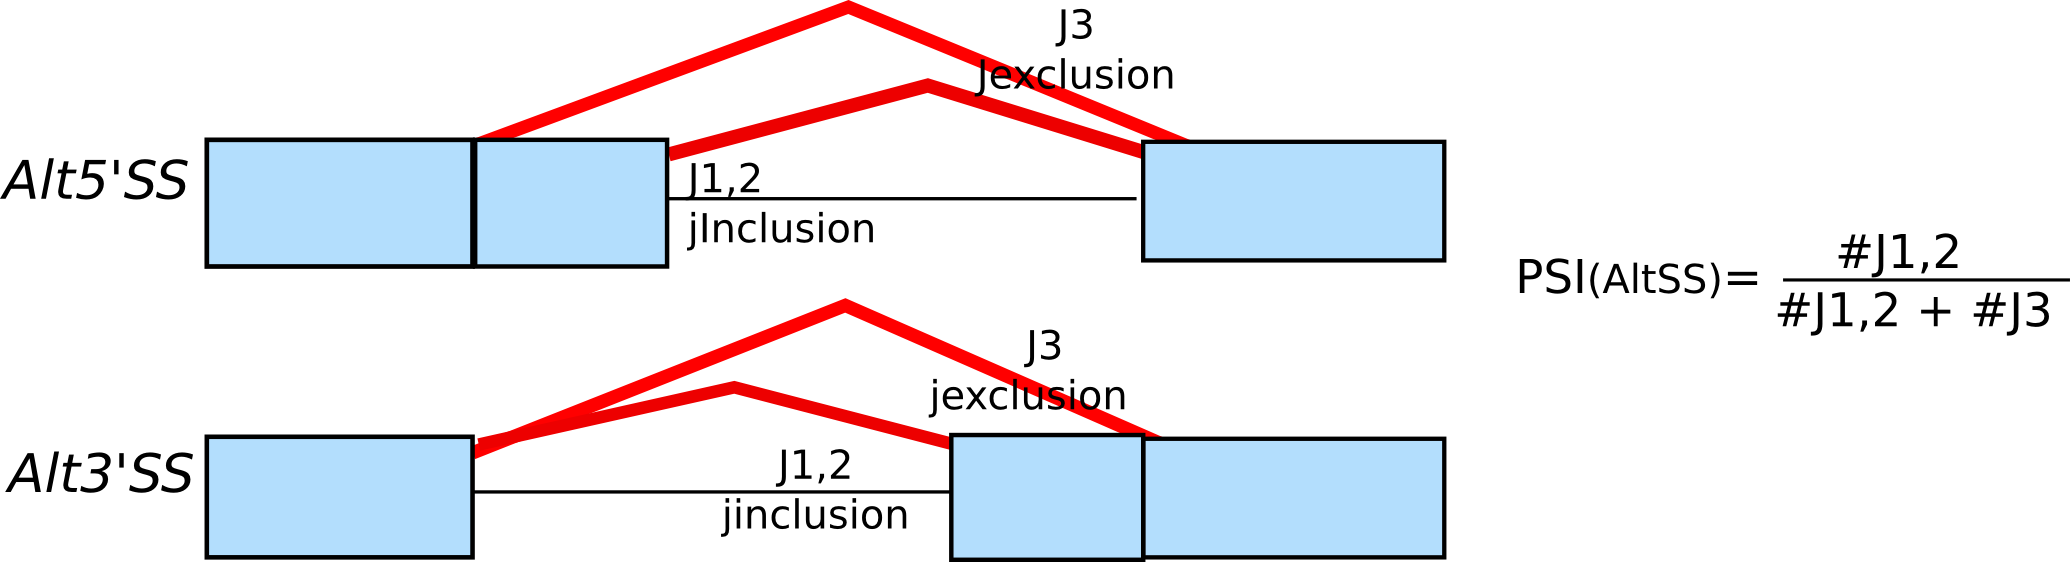
\includegraphics[width=0.5\textwidth]{psi_altSS.png}
      \caption{PSI metric for AltSS estimation and its relationship with junctions}
    \end{subfigure}

\begin{subfigure}[t]{1\textwidth}
\centering
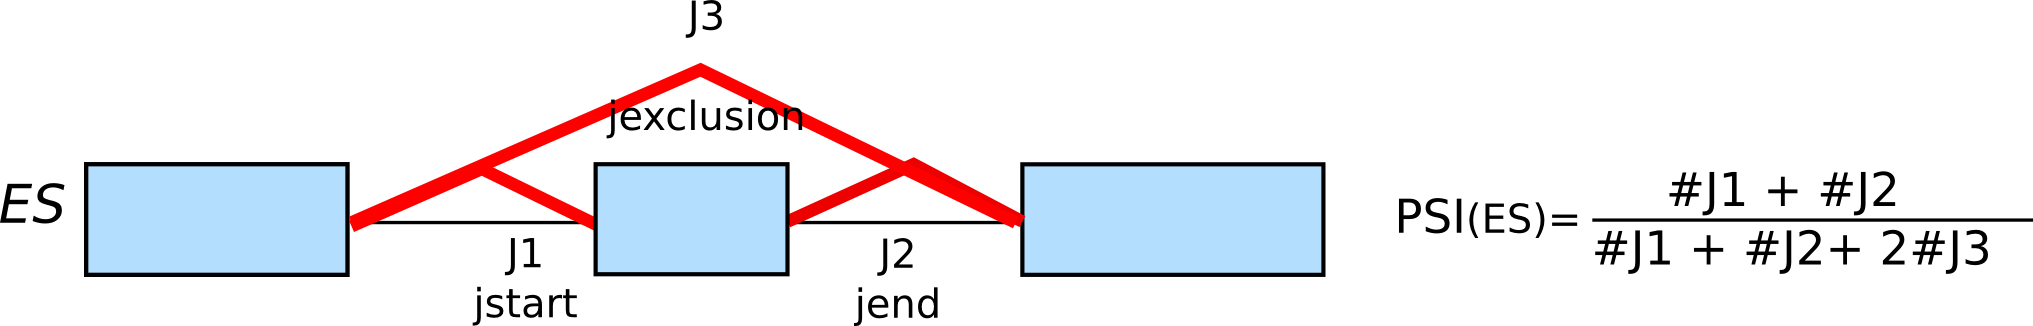
\includegraphics[width=0.5\textwidth]{psi_es.png}
\caption{PSI metric for ES estimation and its relationship with junctions}
\end{subfigure}

\begin{subfigure}[t]{1\textwidth}
\centering
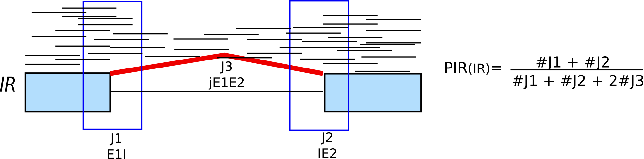
\includegraphics[width=0.5\textwidth]{pir.png}
\caption{PIR metric for IR estimation and its relationship with junctions}
\end{subfigure}
\caption{PSI and PIR metrics estimation and their relationship with junctions}
\end{figure*}

\subsection{Estimating differential gene expression and bin/junction usage}

Using the generated counting tables it is possible to estimate the differential usage (DU) of bins and junctions, and the differential expression at gene level (DE) using any analysis methodology of choice. For the sake of user convinience, we included two wrapper functions, \texttt{DUreport} and \texttt{DUreport\_DEXseq}, that allow to perform such analysis using any of two widespread used methodologies: edgeR and DEXseq, respectively.

DUreport function performs statistical tests using a count centric approach. Results are stored into an \texttt{ASpliDU} object. Individual tables can be accesed using accesors and exported using \texttt{writeDU} function.

<<group, eval=FALSE, echo=TRUE>>=
du <- DUreport(counts, targets)
@

\subsubsection{Differential gene expression (DE)}
Genes are considered expressed if they received in average (parameter \texttt{minGenReads}, default=10)  more than a minimum number of reads  and if average read density per condition is above a threshold in any condition (parameter \texttt{minRds}, default=0.05). Differential gene expression is estimated using edgeR \cite{Robinson2012} package. \textbf{logFC}, \textbf{pvalue}, and \textbf{adjusted pvalue} by false discovery rate \cite{fdr} are reported. 

\subsubsection{Differential junctions and bin usage (DU)}
In order to select informative events the following criteria are adopted:
  
\begin{itemize}
\item \textbf{Junctions}: junctions from expressed genes will be taken into account if they have more reads than a threshold supporting them (parameter \texttt{threshold}, default=5) in one of the conditions. 
\end{itemize}

Where differential junction and bin usage are estimated using the statistical method proposed in the \texttt{edgeR} package, external bins are not included in the analysis (parameter \texttt{ignoreExternal}=TRUE, by default). 
and bin and junction counts are corrected as follow:

Given a \textit{Bin$_i$} belonging to a \textit{Gene$_A$} in condition 1, \textit{Bin$_i$} counts ({G$_A$:B$_i$}) are divided by \textit{Gene$_A$} counts in condition 1 and multiplied by the gene count  average observed along all conditions \~G$_A$

average \textit{Gene counts} in all conditions:

	\[ CountBinAdjusted=(\frac{G_A:B_i}{G_A})_1 * \tilde G_A \]


Output tables can be accessed and exported easily:
 
<<export, echo=TRUE, eval=FALSE>>=
writeDU(du, output.dir="example")
genesde <- genesDE(du)
binsdu <- binsDU(du)
junctionsdu <- junctionsDU(du)
@

\subsection{Output and results}
At each module, results are stored in \texttt{ASpliObjects}. Self-explanatory tables can be exported at each step of the analysis. Using \texttt{write} functions, it is possible to export tab delimited tables in a features-level output folder, as was detailed before:

<<write, echo=TRUE, eval=FALSE>>=
writeCounts(counts, "example_counts")
writeDU(du, output.dir="example_du");
writeAS(as=as, output.dir="example_as");
writeAll(counts=counts, du=du, as=as, output.dir="example_all")
@

Information summary reported in tables:
\subsubsection*{Genomic metadata:}
\begin{itemize}
\item Common info:
    \begin{itemize}
    \item \textbf{locus\_overlap}: whether overlap exists with another gene. Genes with the same coordinates are discarded and only one is kept (first one alphabetically).    
    \item \textbf{symbol}: common name
    \item \textbf{gene\_coordinates}: genomic coordinates in a shrink mode
    \item \textbf{start, end}  and \textbf{length}: genomic coordinate of corresponding feature
  \end{itemize}
%-----------------------------%
\item Gene exclusive 
  \begin{itemize}
  \item \textbf{effective\_length}: sum of length of exons bins of the gene (constitutive and alternative)
  \end{itemize}
%------------------------------%
\item Bin exclusive (exons, introns, e12, ie2 tables):
\begin{itemize}
    \item \textbf{feature}: levels are E (exon), I (intron), Io (original intron)
    \item \textbf{event}: according to our classification, bins are classified into ES, IR, ALt5'SS, ALt3'SS, external. Bins tagged with * means this AS bin is involved simultaneously in more than one AS event type mean they came from 
  \item \textbf{locus}: gene coordinates
\end{itemize}
%------------------------------------------------%
\item Junction exclusive:
  \begin{itemize}
  \item \textbf{junction}: if exist, name of existing junction 
   \item \textbf{gene}: if junction is inside  an existing gene (within)
  \item \textbf{strand}: corresponding strand of gene match
  \item \textbf{multipleHit}: if junction matchs multiple locus
  \item \textbf{bin\_spanned}: bins  spanned by junction 
  \item \textbf{j\_within\_bin}: if junction is included  into a bin. This information is useful for the analysis of possible exintrons. 
\end{itemize}
\end{itemize} 
%----------------------------------------%
\subsubsection*{Junctions metadata:}
The following junction dependant tables with their corresponding content are available (see Figure 3 a,b,c):
\begin{itemize}
\item \textbf{intron.pir}: event, e1i counts (J1), ie1 counts (J2), j\_within (J3), PIR by condition. J1, J2, J3 are the sum of junctions (J1, J2, J3) by condition.
  \[ PIR =\frac{J1+J2}{2*J3+(J1+J2)}\]

\item \textbf{exon.altPSI}: event, J1 (start), J2 (end), J3 (exclusion), PSI. J1, J2, J3 are the sum of junctions (J1, J2, J3) by condition. \\

\[ PSI(AltSS)=\frac{J1,2}{J1,2 +J3)}\]

\item \textbf{exon.altES}: event, J1 (start), J2 (end), J3 (exclusion), PSI. J1, J2, J3 are the sum of junctions (J1, J2, J3) by condition. \\

\[PSI(AltES)=\frac{J1 + J2 }{J1 + J2 +2*J3)}\]

\item \textbf{junctions.pir}: This table is similar to \textbf{intron.pir} table. Contains PIR metric for each experimental junction using e1i and ie2 counts. Exclusion junction is the junction itself. This table helps to discover new introns as well as new retention events. Original data:

\begin{itemize}
\item hitIntron: compares junction with annotated introns
\item hitIntronEvent: reports if the annotated intron is alternative or not
\end{itemize}

\item \textbf{junctions.psi}: Given a junction, we can analyze if it shares start, end or both with another junction. If so, it indicates the existance of an alternative splicing event. Using strand information it is possible to classify those junctions into ALt5'SS, ALt3'SS or ES. Ratio between them along samples is reported.
\end{itemize}  


\subsection{Plots}
Inspection of coverage plots is a good practice for the interpretation of analytical results. After selection of AS candidates it is possible to plot the results in a genome browser manner highlighting  alternatively spliced regions using a simple function \texttt{plotTopTags}.
\begin{itemize}
\item It is neccesary to build an small dataframe (\texttt{auxdf}) with the columns:
\texttt{event, gene\_coordinates, start of bin, end of bin} and bin names as rownames.
\item In \texttt{targetsPlot} object you should specify which BAM files you will plot, in which colors and which sample names you want to display. 

<<targetsPlot, eval=TRUE>>=
bamFiles <- c("CT.bam","KD.bam")
targetsPlot <- data.frame(bam=bamFiles, 
                        sample=sub(".bam", "", bamFiles), 
                        color=c("blue", "black"), 
                        stringsAsFactors=FALSE)
@
\item You have to put \texttt{BAI} files of the corresponding BAM ones in the same folder and provide a \texttt{TxDb} object to the function. 
\end{itemize}

And finally, you can plot:

<<plotTopTags, eval=FALSE>>=
plotTopTags(auxdf, 
            TxDb, 
            targetsPlot, 
            output.dir="testPlots")
@

\section{Example data}
It is possible to run a demo of \texttt{ASpli} using public RNA-seq data available via Bioconductor. It requieres installing of \texttt{RNAseqData.HNRNPC.bam.chr14} package and loading  an small TranscriptDb of Human Genome only for chromosome 14. This subset of reads is part of an experiment intended to analyze splicing factors and their relationship with exonization of Alu elements \cite{Zarnack2013453}. We load the package and the genome:
<<librariesEx, echo=TRUE, eval=TRUE>>=
library(RNAseqData.HNRNPC.bam.chr14)
@

In this case we are loading a genome \texttt{TranscriptDb} already created and available in the  \texttt{ASpli} package for the Homo sapiens chromosome 14:

<<loadDb, echo=TRUE, eval=TRUE>>=
chr14 <- system.file("extdata","chr14.sqlite", package="ASpli")
genome <- loadDb(chr14)
@

And now we are ready to start the complete analysis.
<<binGenome, echo=TRUE, eval=TRUE>>=
features <- binGenome(genome) 
@

Create targets object using the information of the available files:
<<targetsEx, echo=TRUE, eval=TRUE>>=
targets <- data.frame(bam=RNAseqData.HNRNPC.bam.chr14_BAMFILES,
                       condition=c(rep("CT",4),rep("KD",4)))
@
Load bam files:
<<loadBam, echo=TRUE, eval=TRUE>>=
bam <- loadBAM(targets)
@
Overlap alignments against features:
<<todosJuntos, eval=TRUE>>=
counts<-readCounts(features, bam, targets, readLength=100L, maxISize=50000)
@
Perform DE/DU analysis
<<DU, eval=TRUE>>=
du_HNRNPC <- DUreport(counts, targets)
@
Analyze AS using junctions:
<<AS, eval=TRUE>>=
as_HNRNPC <- AsDiscover (counts, targets, features, bam, readLength=100L, threshold = 5, cores = 1 )
@

Select TopTags (only using DU information:)
<<topTags, echo=TRUE, eval=TRUE>>=
binsdu <- binsDU(du_HNRNPC)
topTagsBins <- which(binsdu$bin.fdr <= 0.1 & 
                 abs(binsdu$logFC) >=0.58)
@

We can inspect visually the results of topTags. Sometimes is useful to merge BAM files by conditions. \textit{(In this example data, control and knock down replicates were  merged using \texttt{samtools merge} into \textbf{CT.bam} and \textbf{KD.bam} respectively)}.

<<targetsPlot, eval=TRUE>>=
targetsPlot <- data.frame(bam=targets$bam, 
                        sample=targets$condition, 
                        color=c(rep("blue", 4),rep("red", 4)), 
                        stringsAsFactors=FALSE)
@

<<auxdf, echo=TRUE, eval=TRUE>>=
auxdf<-binsdu[topTagsBins,]
#for simplicity, we choose one: LRR1:E005
plotTopTags(auxdf["LRR1:E005",], 
            genome, 
            targetsPlot, 
            output.dir="testPlots")
@
\begin{figure}[ht!]
\centering
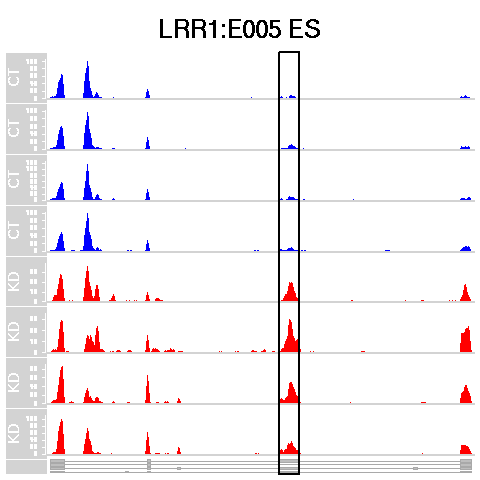
\includegraphics[width=0.5\textwidth]{LRR1_E005.png}
\caption{Plot of LRR1:E005 Exon Skipping}
\end{figure}


<<check, echo=TRUE, eval=TRUE>>=
binsdu <- binsDU(du_HNRNPC)
topTagsBins <- which(binsdu$bin.fdr <= 0.1 & 
                     abs(binsdu$logFC) >=0.58)
@

<<sessionInfo, eval=TRUE, echo=TRUE>>=
sessionInfo()
@

\bibliography{ASpli}
\end{document}
